\begin{figure}[t]
\centering
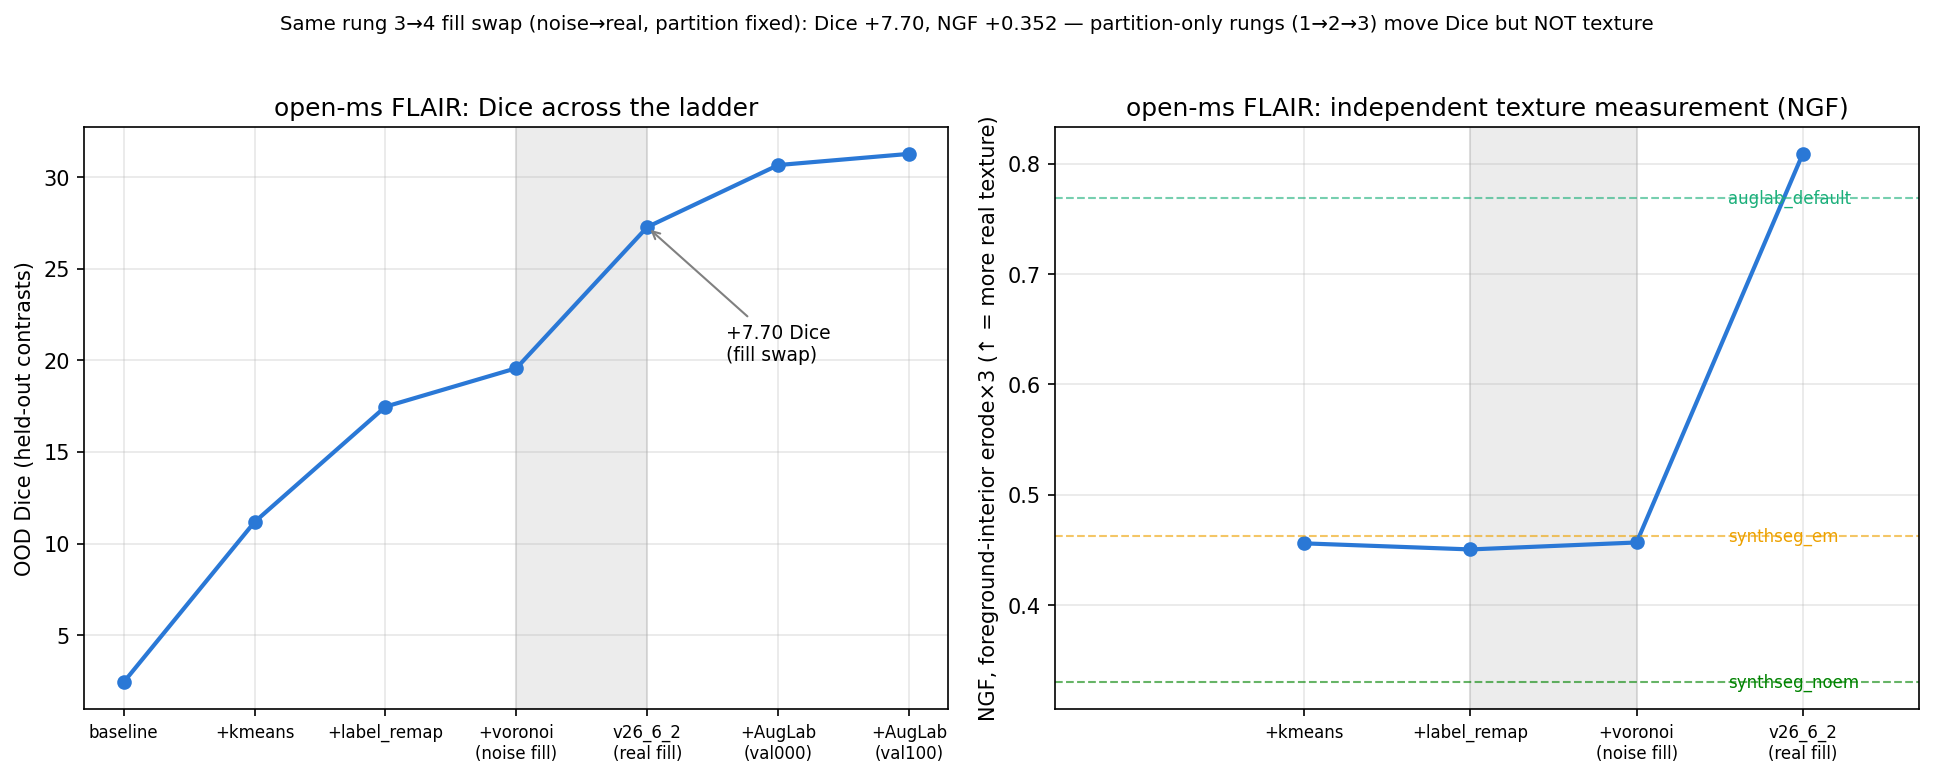
\includegraphics[width=\linewidth]{figures/ngf_dose_response_openms_flair}
\caption{Downstream Dice (left) against an independent, segmentation-free
measurement of texture fidelity (right, NGF gradient-orientation agreement
with the source volume) across the rung sequence. The three noise-fill rungs
sit flat at the texture floor while their Dice still rises -- those gains come
from richer contrast randomization, not texture. Both quantities jump together
at the fill swap, which is the step the texture hypothesis predicts.}
\label{fig:ngf-dose}
\end{figure}

The Dice ablation above
The ablation of \cref{subsec:e-ablation} shows that texture preservation
\emph{matters} downstream; here we measure the texture itself, directly and
without reference to any segmentation.
For each method we compute the normalized-gradient-field (NGF)
similarity~\cite{haber2006ngf} between the augmented image and the source
scan --- an alignment-of-gradients measure that is high when local edge and
texture structure is retained and near the isotropic-noise floor
($\approx\!1/3$) when it is destroyed. \cref{tab:ngf} reports mean NGF over
$n{=}30$ scans on the two Open-MS contrasts. PALETTE retains far more of the
source texture than any noise-based method and significantly more than
Auglab (FLAIR $p=7.6\times10^{-3}$, T1w $p=1.2\times10^{-6}$), while the
label-style methods (SynthSeg-EM, noise-fill) and especially SynthSeg-noEM
sit near the noise floor --- exactly the ordering the mechanism predicts, and
consistent with the downstream Dice gaps of \cref{tab:dissociation}.

\begin{table}[t]
\centering
\small
\setlength{\tabcolsep}{6pt}
\begin{tabular}{lcc}
\toprule
Method & FLAIR & T1w \\
\midrule
\textbf{PALETTE} & \textbf{0.808} & \textbf{0.894} \\
Auglab           & 0.772 & 0.777 \\
SynthSeg-EM      & 0.461 & 0.422 \\
noise-fill       & 0.453 & 0.401 \\
SynthSeg-noEM    & 0.332 & 0.319 \\
\bottomrule
\end{tabular}
\caption{Texture fidelity measured by NGF similarity to the source scan
(mean over $n{=}30$ Open-MS scans; higher = more source texture retained,
$\approx\!1/3$ = isotropic-noise floor). PALETTE preserves the most texture;
the noise-based methods sit near the floor.}
\label{tab:ngf}
\end{table}
